\documentclass[]{final_report}
\usepackage{graphicx}
\usepackage{hyperref}
\usepackage[dvipsnames]{xcolor}
\usepackage{verbatimbox}
\usepackage{multirow}
\usepackage{tabularx,booktabs}
\usepackage{mathtools}
\newcolumntype{Y}{>{\centering\arraybackslash}X}
\usepackage[skip=2pt,font=normalsize]{subcaption}
\usepackage[skip=2pt,font=normalsize]{caption}
\usepackage{enumitem}
\setlist{nosep}
\usepackage{xfrac}
\usepackage{array}
\newcolumntype{P}[1]{>{\centering\arraybackslash}p{#1}}
\newcolumntype{M}[1]{>{\centering\arraybackslash}m{#1}}
\renewcommand{\arraystretch}{2}
\usepackage[toc,titletoc,title]{appendix}
%TC:group tabular 1 1
%%%%%%%%%%%%%%%%%%%%%%
%%% Input project details
\def\studentname{Natalia Kenrick}
\def\reportyear{2022/23}
\def\projecttitle{Single-Agent and Multi-Agent Search in Maze Games}
\def\supervisorname{Farid Shahandeh}
\def\degree{BSc (Hons) in Computer Science}
\def\fullOrHalfUnit{Full Unit} % indicate if you are doing the project as a Full Unit or Half Unit
\def\finalOrInterim{Interim Report} % indicate if this document is your Final Report or Interim Report

\begin{document}

\maketitle

%%%%%%%%%%%%%%%%%%%%%%
%%% Declaration

\chapter*{Declaration}

This report has been prepared on the basis of my own work. Where other published and unpublished source materials have been used, these have been acknowledged.

\vskip3em

Word Count: 5271

\vskip3em

Student Name: \studentname

\vskip3em

Date of Submission: 01/12/12

\vskip3em

Signature:\par\medskip
\includegraphics[height=2\baselineskip]{Dissertation/Interim Report/Pictures/signature.pdf}\par 

\newpage

%%%%%%%%%%%%%%%%%%%%%%
%%% Table of Contents
\tableofcontents\pdfbookmark[0]{Table of Contents}{toc}\newpage

%%%%%%%%%%%%%%%%%%%%%%
%%% Your Abstract here

\begin{abstract}
The aim of the project is to implement general search algorithms to single and multi-Agent environments in order to find the optimal route through a maze and to complete some goal. By designing and implementing agents with different goals, each will need to find efficient ways through the maze in order to complete their goal.

This project is intriguing because it shows how we can use autonomous agents to complete some task without user input. This is especially interesting in a multi-Agent scenario where agents can communicate and help each other to reach their goal. 

In order to implement the search algorithms to our maze, we will model the maze as a search problem. By using simple uninformed search algorithms such as depth-first search and breadth-first search, we can find a specific location in a maze. Later, we can introduce a cost function to our search to find the shortest distance. We can also apply more complex search algorithms, such as the A* algorithm, which uses a heuristic in order to better inform our agent of its surroundings. By combining different search algorithms, we can produce the most optimal outcome for our goal.
\end{abstract}
\newpage

\chapter*{Project Specification}
\addcontentsline{toc}{chapter}{Project Specification}

%TC:ignore
\begin{minipage}{\textwidth}
\textbf{Aims:} The goal of this project is to implement general search algorithms and apply them to single-agent and multi-agent scenarios in maze games (e.g. Pac-Man).

\textbf{Background:} Maze games are a video game genre in which the entire playing field is a maze. Usually, the player needs to navigate the maze to collect items and also performs other actions (e.g. escape monsters and outrace an opponent) within a time limit. The most popular example is Pac-Man by Namco (1980), but many other maze games exist. You will model a maze game as a search problem and then design and implement agents that inhabit the maze. The agents will find efficient paths through the maze world, to reach a particular location, to collect food and to combat opponents.

\textbf{Early Deliverables}

\begin{enumerate}
    \item Given a maze game of your interest (e.g. Pac-Man), design and implement a simple graphical visualisation for it.
    \item Consider an agent inhabiting the maze world. Model the agent's navigation task as a search problem. Implement a graph search version of depth-first search and breadth-first search to reach a specific location in the maze. Run experiments with three different size maze: small, medium and large. Visualise the agent following the plan step-by-step.
    \item Now change the cost function in such a way that traversing some areas is more expensive than traversing other areas (e.g. Pac-Man: you can charge more for dangerous steps in areas close to the ghosts). Implement the uniform-cost graph search algorithm to reach a specific location in the maze. Run experiments with three different size maze: small, medium and large. Visualise the agent following the plan step-by-step.
\end{enumerate}

\textbf{Final Deliverables}

\begin{enumerate}
    \item Implement the algorithm A* to find the shortest path through the maze that touches all four corners. Use two different, consistent heuristic functions. Run experiments with three different size maze: small, medium and large. Visualise the agent following the plan step-by-step.
    \item Assume each cell in the maze has an item to collect. Formulate a search problem for collecting all items (e.g. in Pac-Man: eating all the food) and implement A* to do that in as few steps as possible. Also implement a greedy search and compare the results of the two algorithms in three different size maze: small, medium and large. Visualise the actions of the agent.
    \item Now assume that you have additional agents in your maze, one is the main player and the other are the opponents (e.g. Pac-Man and the ghosts). Model this new problem and implement the player as a reflex agent that tries to visits all cells avoiding the opponents.
    \item Implement an adversarial Minmax search agent for each agent; start with the player and one opponent and then increase the number of opponents. You need to write an evaluation function that evaluates states. Run experiments with three different size maze: small, medium and large. Visualise the actions of the agents.
    \item Design and implement a new agent that uses Alpha-beta pruning to more efficiently explore the minimax tree. Run experiments with three different size maze: small, medium and large. Visualise the actions of the agents.
    \item Design and implement an Expectimax agent to model the probabilistic behaviour of an agents who makes suboptimal choices. Run experiments with three different size maze: small, medium and large. Visualise the actions of the agents.
\end{enumerate}

\textbf{Suggested Extensions}
\begin{itemize}
    \item Use value iteration and Q-learning to underpin the behaviour of the player.
\end{itemize}
\end{minipage}
%TC:endignore

%%%%%%%%%%%%%%%%%%%%%%
%%% Introduction
\chapter{Introduction}

\section{Idea}

When developing large systems with many smaller sub problems, sometimes using functional programming, or even object oriented programming, can be difficult. Multi agent systems can be incredibly useful when used to decompose a difficult problem into lots of small sub problems. 

A multi-agent system is a society of distributed autonomous, cooperative entities\cite{leitao2013multi} in which each agent has its own goal, knowledge base and agent program   (further details in section \ref{Agents and Environments}).

An example of how we can implement a multi-agent system could be planning a traffic route for hundreds of self driving cars. This problem would be nearly impossible if executed functionally. However, if we were to approach this problem in the multi-agent paradigm, we can abstract the problem into manageable pieces. If we turn each car in this instance into an agent, with its own set of instructions to follow, then suddenly we aren't dealing with hundreds of cars, we can focus on how to make a single agent get to its destination, and how it should interact with others as it does. 

One real world example of how a multi-agent systems can be implemented is SARDINE (System for Airline Reservations Demonstrating the Integration of Negotiation and Evaluation). SARDINE uses agents to coordinate preferences and interests of a buyer. The buyer agent takes this information and correlates these to available flights from a reservation database. The user then informers the buyer agent on how much it should bid. The airline agents accept the ticket bids from the buyer agent. Finally, the airline agents consider
individual bids based on flight yield management techniques and specific buyer information\cite{oprea2004applications}.

We want to use agents as they are extremely useful tools that can be used in many different types of applications. Often, they are implemented to act as an extension of the user. By this we mean that they provide some service to the user that would otherwise take prove time consuming id completed themselves e.g. browsing the internet for specific files. We can use an agent to do this task; It will work continuously without getting tired or distracted, and can be programmed to only gather information that is known to be useful for the user\cite{jennings1996software}.  

\section{Aims and motivations}

The aim of this project is to show how we can use agents to solve problems autonomously. More specifically, we will be demonstrating how agents can navigate their way through a maze using search algorithms, in both single and multi-agent scenarios. By visualising the routes they take we can display how they change their behaviour based on the goal they wish to achieve. 

We use search algorithms to find the shortest path. They can be used in many ways, including complex issues such as optimal energy efficient path planning for an unmanned air vehicle\cite{debnath2019review}. We aim to implement two forms of search algorithms, uninformed and informed. Informed searches are more efficient then uninformed searches as they have more information about the problem itself and are able to use methods such as heuristics functions to work out the optimal path. 

By the end of this project, we hope to showcase how the use of intelligent agents can be used to automate tasks by displaying how their decision making movements occur in a game-like scenario. 
\newpage
\section{Milestones}

\begin{center}
\begin{tabular}{||c|M{0.15\linewidth}|m{0.55\linewidth}||} 
\hline
 Deliverables & Milestone & \multicolumn{1}{c||}{Why it's important}\\
\hline\hline
\multirow{8}{*}{Implemented} & Create maze generation and visualisation & We will be deploying our agent in a maze. This will be its environment. We need to be able to see a graphical visualisation of the maze in order to display our agent's movement\\\cline{2-3}

    & Create graph representation of our mazes & We need to model our mazes as search problems. To do this, we imagine the maze as a graph, with nodes and edges. We can then represent this in our code in order for the agent to be able to perform.\\\cline{2-3}
    
    & Create a problem solving agent (\ref{Agents and Environments}) & We need an agent that can hand its problem to an algorithm, for an uninformed search this is a path that reaches a goal. It can then execute the returned action sequence\\\cline{2-3}
    
    
    & Implement uninformed searches & To be able to visualise the journey the agent takes, it needs to receive an action sequence. Each uninformed search we visualise will return the appropriate action sequence to our agent. \\

\hline\hline

\multirow{12}{*}{\parbox{0.15\linewidth}{\centering Future Deliverables} }& Create Heuristic Functions & The final single agent visualisation step is to implement informed searches. In order to do this we will need to create heuristic functions for the algorithm to implement.\\\cline{2-3} 

   & Implement informed searches & By now we have seen how uninformed searches behave, the logical next step is to visualise how informed searches behave, using our heuristic functions.\\\cline{2-3}
   
   & Add additional agents & We want to show how multi-agent systems behave. To do this we want to add extra agents that act as 'baddies' into our game, as well as keeping our main player. We will need to find the most optimal type of agent for this scenario.\\\cline{2-3}
   
   & Implement an adversarial Minmax search & Once we have a multi-agent scenario working, we want to increase the complexity of our system to really display the capabilities of agents in a multi-agent scenario. One way to display this is by applying a Minmax search to multiple agents and commenting on the effects this has. \\\cline{2-3}
   
   & Implement different types of agents & One we have the base of a multi-agent system (we understand how to implement the agents and their interactions), we can begin experimenting with deploying different types of agents and see how these new agents effect the 'gameplay'.\\
   \hline
\end{tabular}
\end{center}

\newpage
\chapter{Background}
\section{Agents and Environments}\label{Agents and Environments}

To understand what a multi-agent scenario entails, first we have to understand what an agent actually is. An agent is something that can perceive its environment through sensors and can complete some autonomous action through actuators in said environment. They are comprised of two properties, an agent function and an agent program. The agent function maps actions to percepts; It decides what action the agent should perform given the current percepts. The agent program is the execution of the agent function. 

A multi-agent system will use intelligent agents. According to Wooldridge\cite{WooldridgeMichael2009AitM}, an agent is considered intelligent if it has the following characteristics: reactivity, pro-activeness and social ability. What we mean by this is that an agent is able to react to changes in the environment in a timely fashion, make decisions based on their goal and can communicate with other agents.

We mentioned before that agents are very useful tools. For example, they scale a lot better than objects, which do not have autonomy over their actions (Kostas Stathis 2022). We can think of agents as active objects that have initiative. They require less organisation on implementation when compared to objects as they can organise themselves. Let's imagine we have many agents completing some task, if one fails, the impact on the system as a whole may be minimal, but if an object fails an exception is raised.\cite{odell2002objects}.

To be able to use an agent, it needs to be situated in an environment. Environments can have different characteristics. When implementing uninformed searches, our environment will be:

\begin{itemize}
    \item \textbf{Observable/Accessible:} Our agent always knows the state of the environment.
    \item \textbf{Discrete:} From any state, all possible actions are known and finite.
    \item \textbf{Deterministic:} Each action has only 1 known outcome.
    \item \textbf{Static:} The environment remains unchanged, accept from actions performed by the agent.
\end{itemize}

A multi-agent system uses many intelligent agents of same or different types in order to achieve some task/goal. We can now see how the characteristics of intelligent agents become important. This is because in order to complete their combined goal, they need to be able to communicate and react to other agents, whilst making sure to stay focused on their own individual goals. An example to intelligent agents working together is the very well know scenario Vacuum World. Let's say we have two agents, Orange and White. Their combined goal is to make sure there is no dirt in the environment. Their individual goal is to clean up dirt of their own colour. In this scenario, the white agent can communicate to the orange agent where it has seen orange dirt, and vice versa (social ability). The orange agent can react to this message by heading toward the known dirt location (reactivity and pro-activeness).

There are many different types of agents, each with their own characteristics making them suitable for different goals. Some agents have a knowledge base, a set of facts/beliefs about the environment.  So far in this project we have used goal-based agents, as well the mention of a simple reflex agent in section \ref{unininformed search implimentation}.

A \textbf{goal based agent's} decisions are based on whatever gets it closer to its goal. At each state, it needs some sort of information to do with the goal in order to pick the action that is the most desirable. We will use a type of goal based agent called a problem solving agent. This problem solving agent is used when showcasing \textit{uninformed searches}. This type of agent is used because it doesn't care about the internal structure of the states. The uninformed search will take the problem as an input and return and action sequence for the agent to then carry out. By doing this, the agent is ignoring all of its precepts, therefore best used in a static environment where nothing will change except by actions of the agent\cite{russell2016artificial}.

A \textbf{simple reflex agent} is the most simple agent to use. They choose their actions based on their current percept, they do not have a history of past actions or percepts. A simple reflex agent is only able to perform actions in a fully observable environment. This is because they work by reacting to their current percepts, without them they do nothing. They are most useful on small environments performing basic experiments (Kostas Stathis 2022).

We will see later in section \ref{Finding Goals} how these agents work when implemented to find a goal in a maze. 

\newpage
\section{Search Algorithms}\label{Search Algortithms}

The next main component of our project is search algorithms. The final goal is to use both informed and uninformed searches. This paper concentrates on the search that has been implemented so far, uninformed searches.

We will need to model the maze as a search problem in order to apply these algorithms. Wolfgang Ertel\cite{Ertel_2011} states that a search problem can be defined by having the following properties:

\begin{itemize}
    \item \textbf{State:} The state of the world the agent is in
    \item \textbf{Start State:} Initial state of agent
    \item \textbf{Goal state:} The goal state of the agent, where it terminates and returns a solution
    \item \textbf{Actions:} The actions our agent can take
    \item \textbf{Solution:} Path taken or to be taken by our agent
    \item \textbf{A cost function:} Cost value of action (path cost). In the case of no path cost, each action has an equal value
    \item \textbf{State Space:} Set of all states
\end{itemize}

We will use this design when modelling our problem.

\subsection{Uninformed Search}\label{Uninformed search} 

An uninformed search (also known as blind search) does not hold any information about the number of steps to reach the goal. It only considers which path is most promising at a point in time, but not the most optimal\cite{pathak2018comparative}. These searches only know whether or not the current state is or isn't the goal state. They expand every node in a brute-force kind of way. Uninformed search algorithms take our agents problem as an input and returns the solution in the form of an action sequence \cite{russell2016artificial}.

\subsubsection{Breadth-first Search}\label{Breadth-first Search}

A breadth-first search (BFS) is a simple uninformed search that works by expanding all nodes at the same depth level, before moving onto the next level. A BFS uses a first-in-first-out (FIFO) queue when expanding nodes. This is quite inefficient as goals on the bottom level are expanded last. A BFS does not consider path cost when expanding nodes, it is best used on a graph with equal or no path costs.

The steps of performing a BFS are:

\begin{enumerate}
    \item Add initial state to an explore list \textbf{E}
    \item Take the first item in the list \textbf{X}, add to list of visited states, \textbf{V}
    \item If \textbf{X} is our goal, stop. Else
    \item Find all children of \textbf{X}.
    \item If children of \textbf{X} do not appear in either \textbf{E} or \textbf{V}, add child to end of \textbf{E}
    \item Repeat from step 2 until list \textbf{E} is empty
    \item Return \textbf{V}
\end{enumerate}

Time complexity is the computational complexity which describes the time taken for an algorithm to run. For a BFS, this is $O(|V| + |E|)$ where $|V|$ represents the number of vertices and $|E|$ represents the number of edges. However, if we were to be working in a tree of infinite size, the running time can be written as $O(b^d)$. The reason for this is because if we have a tree of infinite size, we do not know the number of edges or vertices per say. $b$ represents the branching factor, the number of children at each node ($b$ = maximum branching value, its the worst case). $d$ represents the depth of the shallowest solution. One can think of this as looking $d$ steps ahead.

\subsubsection{Depth-First search} 

A depth first search (DFS) is another example of a simple uninformed search. It expands a node all the way to its deepest child, before returning to the next deepest node and expanding that all the way etc. A depth first search uses a Last-in-first-out (LIFO) queue, opposite to a BFS. This means it's always expanding the deepest unexpanded node. Like a BFS, a DFS does not consider path cost when expanding nodes. We will be using the DFS on a graph structure, meaning there is a finite number of nodes for it to expand; however, let's say we were working on an infinite binary tree, if our goal state is the first node on the right but we expand the left side first, we will never reach our goal as it will keep expanding the deepest node forever. If this was the case, we could use a depth-limited DFS (Depth-limited search), see \ref{Depth-limited search}.

Steps for performing a DFS:
\begin{enumerate}
    \item Add initial state to a explore list \textbf{E}
    \item Take the last item in the list \textbf{X}, add to list of visited states, \textbf{V}
    \item If \textbf{X} is our goal, stop. Else
    \item Find all children of \textbf{X}.
    \item If children of \textbf{X} do not appear in either \textbf{E} or \textbf{V}, add child to end of \textbf{E}
    \item Repeat from step 2 until list \textbf{E} is empty
    \item Return \textbf{V}
\end{enumerate}

Notice this is almost identical to The BFS shown in \ref{Breadth-first Search}, only this time we expand the last item. This can however be done recursively, with no significant improvement on running time (but looks nicer, \ref{fig: recursive dfs}). 

\begin{verbbox}
def RecursiveDFS(node, path):
    path.append(node)
    for each child of node:
        if node not in path:
            RecursiveDFS(child, path)
\end{verbbox}
\begin{figure}[ht]
  \centering
  \theverbbox
  \caption{Pseudocode for recursive DFS}
  \label{fig: recursive dfs}
\end{figure}


The running time for a DFS is $O(|V| + |E|)$, same as a BFS. In the case of an infinite tree, the running time is $O(b^m)$ where $b$ is the branching factor and $m$ is the maximum depth.

\subsubsection{Depth-limited search} \label{Depth-limited search}

When trying to find a goal in a DFS we want to make sure we are not looking any deeper than we need to. If we know that the goal is withing the first \textit{d} levels of our tree/graph then we can set a limit to out DFS. This is called a depth-limited search. A depth-limited search works the same as a DFS but assumes nodes at depth \textit{d} has no children. If we don't know where the goal is, we can perform and \textbf{iterative deepening search}, which increases the depth \textit{d} until we find the goal. The running time is $O(|V| + |E|)$, same as a BFS. In the case of an infinite tree, the running time is $O(b^l)$ where $b$ is the branching factor and $l$ is the depth limit.

\subsubsection{Uniform-cost search}

As stated earlier in the chapter, A BFS performs best on a graph with equal or no path cost. But when we do have a path cost, BFS is significantly less optimal. To build on this idea of expanding outwards rather than downwards (DFS), we can use a Uniform-Cost Search (UCS). A UCS expands the node with the lowest path cost each turn. To do this, it uses a priority queue. Unlike a BFS, it is possible to store the goal in the queue and not say we have found it. This is because it is still a possibility that we will find a shorter path to the goal when expanding other nodes. The goal is only said to be found if it is chosen from the priority queue, meaning there is no shorter path to be found. 

When adding to the priority queue it may be that we find a shorter path to a node which is already in our queue. If this is the case, we can update its path cost and therefore reposition it in the queue.

Steps for performing a DFS:
\begin{enumerate}
    \item Add initial state to a priority queue \textbf{P}
    \item Take item with highest priority (lowest path cost) \textbf{X}, add to a list of visited states \textbf{V}
    \item If \textbf{X} is our goal, stop. Otherwise,
    \item Find all children of \textbf{X}, with path cost priority of \textbf{X} + path cost to child
    \item If children of \textbf{X} do not appear in either \textbf{P} or \textbf{V}, add child to \textbf{P}
    \item If child is in \textbf{P} with higher path cost, update priority of child in \textbf{P}
    \item Repeat from step 2 until goal is found or P is empty
    \end{enumerate}
    
The running time for a UCS is $O(b^{\lfloor 1+\sfrac{C}{\epsilon} \rfloor})$. Here, $C$ is equal to the cost of the optimal solution. We are assuming every action cost at least $\epsilon$.\cite{pathak2018comparative}. A uniform cost search has a worse running time that a BFS if it is applied to a problem where all edges are the same. This is because it includes an extra step at the end to check if it's the goal node. In a BFS we stop when we find the goal, in UCS we stop when we select the goal node to be expanded.\cite{time-complexity}

The next chapter will show how we can bring all these ideas together, visualising the agent's steps as it completes these algorithms.

\chapter{Implementation}
\section{Maze}\label{Maze implimentation}

The first step for implementation is to design a maze. In order to generate the maze randomly some research was done about maze generation. A useful tutorial\cite{maze} which explained how to generate a perfect maze (a maze with no cycles) was used to help get started. Once this implementation was understood, it was used as the base for the maze generation. After generating a few random mazes, there was a realisation that it would be difficult to get fair experiment results with different algorithms if they were not able to be applied to identical mazes. To fix this issue, the generated mazes were saved as two-dimensional arrays so that they could then be reloaded and reused. To do this we use a maze object. The maze object takes the requested dimensions of the maze as parameters, and a two-dimensional array; this way, a new maze is only generated if the maze parameter is empty, otherwise it loads the saved maze.

\begin{figure}[h]
     \centering
     \caption{Maze generation}
     \begin{subfigure}[h]{0.3\textwidth}
         \centering
         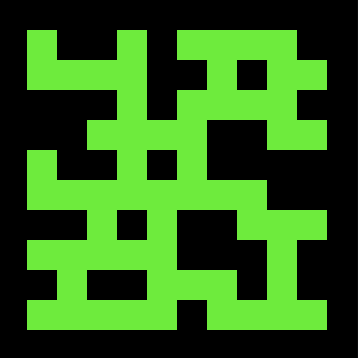
\includegraphics[width=1\textwidth]{Dissertation/Interim Report/Pictures/small.png}
         \caption*{Small: 12 x 12}
     \end{subfigure}
     \hfill
     \begin{subfigure}[h]{0.3\textwidth}
         \centering
         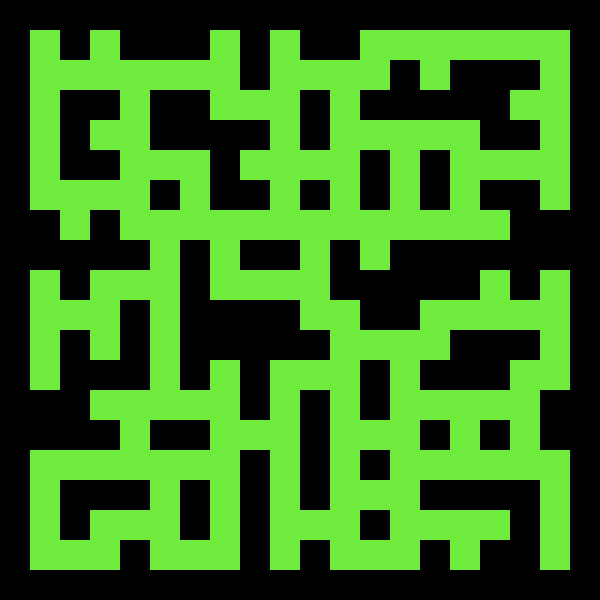
\includegraphics[width=1\textwidth]{Dissertation/Interim Report/Pictures/Medium.png}         \caption*{Medium: 20 x 20}
     \end{subfigure}
     \hfill
     \begin{subfigure}[h]{0.3\textwidth}
         \centering
         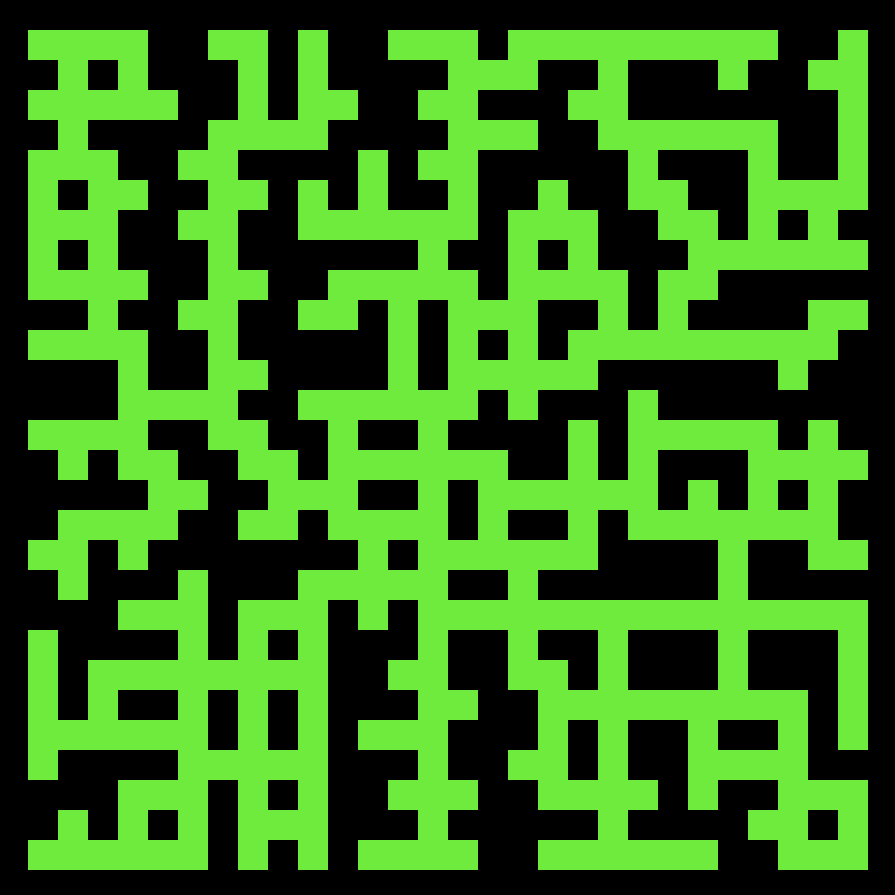
\includegraphics[width=1\textwidth]{Dissertation/Interim Report/Pictures/large.png}
         \caption*{Large: 30 x 30}
     \end{subfigure}
\end{figure}

The smallest maze we have is 12 x 12 cells. Originally the idea was to have the maze sizes going up in tens, however by having a maze size of 10 x 10 there was only 1-2 cycles at most. It was decided that a maze with more cycles would be a better way to showcase the algorithms, so the dimensions were changed to be 12 x 12. The largest maze is 30 x 30. These dimensions are large enough to showcase the agent and algorithms without wasting time repeating similar actions on a large scale.

The mazes are stored in 2D arrays, each element representing a row in the maze. This means when selecting a location on the maze, say for a goal, it has to be in the form (y, x). Storing the maze in this way is more understandable when working with the code from a programmer's perspective.

The goal of this project is to display how an agent behaves whilst trying to achieve some goal so this reason the representation of agents and goals were made to be very simple. An agent in the maze is represented by a blue square. Goals are represented with a red square.

In order to model the maze as a search problem, we have a class to turn the maze into a graph representation. An attempt was made to show a visualisation of the maze using networkx and matplotlib (python libraries), however it didn't appear helpful, see appendix \ref{Graph visualisation} for more details. The graph is represented as a dictionary with the 2D-array coordinate as the key, the value being an array containing each child, the distance to the child and the steps to reach the child. It was important to add the steps to reach the child node otherwise the agent would not be able display these steps throughout its execution of the algorithms. A point in the maze is identified as a node if it has exactly 2 two children. A point with exactly 2 children is simply the path taken between 2 nodes. A point with one child is a leaf node. In figure \ref{Nodes} the cells identified to be a node have been highlighted in purple.

\begin{figure}[h]
     \centering
     \caption{Nodes within maze}
     \begin{subfigure}[h]{0.45\textwidth}
         \centering
         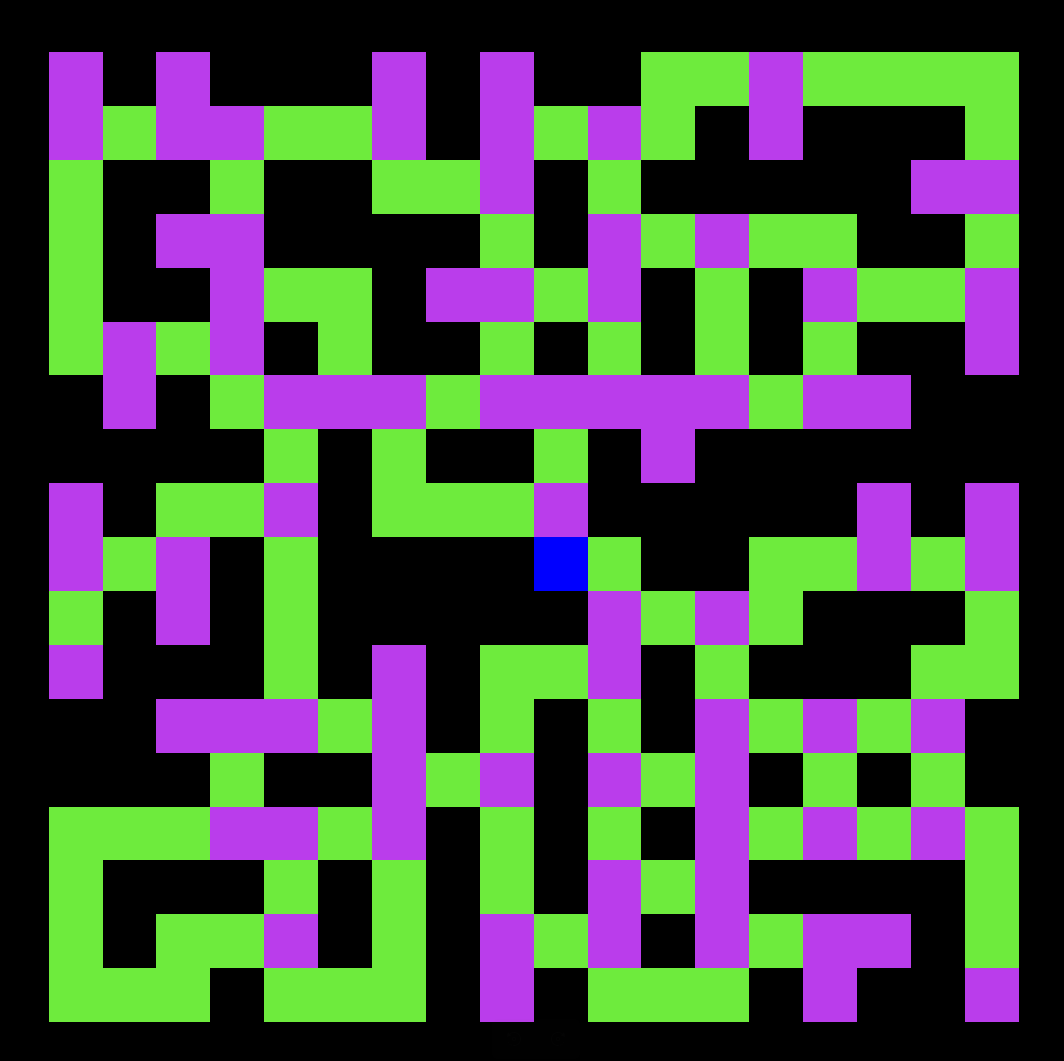
\includegraphics[width=1\textwidth]{Dissertation/Interim Report/Pictures/Nodes.png}
         \caption*{Identified nodes on maze}
     \end{subfigure}
     \hfill
     \begin{subfigure}[h]{0.45\textwidth}
         \centering
         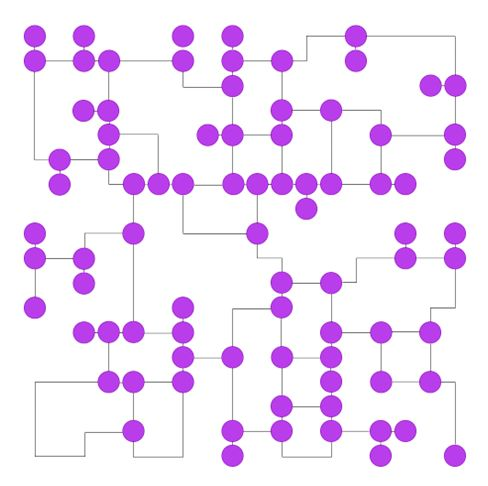
\includegraphics[width=1\textwidth]{Dissertation/Interim Report/Pictures/Graph.jpeg}
         \caption*{Graph representation}
     \end{subfigure}
     \label{Nodes}
\end{figure}

\textbf{Uninformed Search}

Now that we have our maze, we need to write the algorithms for uninformed searches. Test Driven Development (TDD) was used when writing the uninformed searches. To do this, a library called unittest was used, which when ran from the command line informs you which tests failed or passed. A test maze was created and saved so that we were able to check that the algorithms were returning the expected values.

When implementing the UCS a priority queue was not used, that is, a priority queue class was not created and implemented into the algorithm. Instead, we use a function that returns the item with the highest priority (lowest path cost). This was done for two reasons. 
\begin{itemize}
    \item The first reason was because the graph is stored in a way that passing all the values to a priority queue seemed inefficient as they would have to be rearranged in a conflicting way to the other lists.
    \item The second reason was in creating a priority queue, we would have to create the same function in order to pop the item with the highest priority, therefore by not explicitly creating a class priority queue, we could be more efficient with my time.
\end{itemize}
  It should be noted however that by not creating a priority queue we then needed our own function for updating values, which would have also been included in a priority queue class. If this situation were to happen again, creating a priority queue may be tidier.

\subsection{Software Engineering}

As mentioned above, TDD was used when implementing the search algorithms. TDD is a form of unit testing that forces the programmer to build from the bottom up. First, they should create a test to fail. Next they should write just enough code for the test to pass. Then They should test again with different values. At this point the test should fail again, and the programmer can then refactor and re-write the code so that it will pass the tests. This way the programmer is sure that this method works correctly. This is known as red-green-refactor-commit. By commit, it is assumed that the programmer is using some for of revision control system (As any good programmer should). The use of TDD was fairly difficult on this project as a lot of the testing was visual. We were able to \textit{see} that the code was being visualised correctly, but could not use TDD to test this. We could however use it on the search algorithms as we know where it should start, where is should visit next, where is should finish and how many steps it should've taken. By using TDD we were able to ensure that the algorithms were behaving correctly. 

Revision control systems are extremely useful when working on code - especially if there are multiple people working on the same project. This system allows users to checkout a version of the project into their own branch. Here, any changes made to the project will not effect any other user. Once a specific task or goal has been implemented, the user can merge back to the main branch, where everyone can now access these changes. A revision control system is also a good tool as it allows users to work on multiple devices, and means that they do not have to worry about losing the code as it is all stored online. 



\chapter{Experiments}
\renewcommand{\arraystretch}{1}
\section{Uninformed Searches}\label{unininformed search implimentation}

As seen in section \ref{Search Algortithms}, we have a few types of uninformed searches we can use when traversing through the maze. You will now see a selection of experiments, all done on the same machine with the same parameters so that the experiment can be considered to be fair. These experiments will show how long each search took to reach the goal. Each search was run 3 times to get the average time taken, we did not use any time delay in the code. As explained in the section \ref{Maze implimentation}, each node/goal is in the form (y, x). All times have been rounded to four decimal places. The mazes used for testing were randomly generated and then saved so that they could be reused for all searches. It should be noted, the time recorded includes the time taken to visualise the algorithm. This was done as the aim was to show how long the \textit{agent} takes to traverse the maze, not how fast the algorithm itself takes.

When implementing uninformed search algorithms, we need to make sure we use the right agent. As we have a \textbf{goal} for our agent, we know it will be a type of goal-based agent. More specifically, the type of goal-based agent will be a problem-solving agent as described in \ref{Agents and Environments}. It would be possible in the case of a uniform-cost search to use a simple reflex agent. This would be a suitable option because it chooses path of least cost at each step i.e. only cares about its current percepts, however, as our environment is static it is just as efficient to use a problem-solving, goal based agent as before.

When looking at the time complexity of our algorithms, as described in section \ref{Uninformed search}, we would expect a DFS and BFS to run in roughly the same time. It's to be expected that our depth-limited DFS would out perform the DFS in the cases where $l < m$. Our UCS should perform better than our BFS because, although it branches out similar to the BFS, it ignores edges with large costs. As a hypothesis, we expect the depth-limited search to outperform the DFS, and the UCS to do better on average then the BFS. 

\subsection{Finding Goals}\label{Finding Goals}
%%%%%%%%%%%%%%%%%%%%%%%%%%%%%%%%%%%%%%%%%%%%%%%%%%%%%%%%%%%%%%%%%%%%%%%%%%
\textbf{First Experiment: Goal about mid-way through maze}
\begin{figure}[h]
     \centering
     \begin{subfigure}[h]{0.3\textwidth}
         \centering
         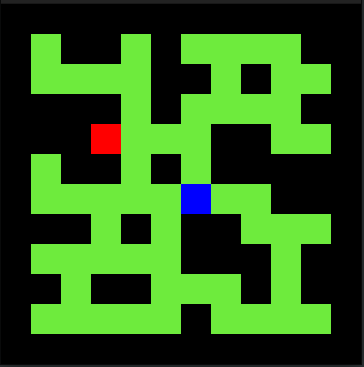
\includegraphics[width=1\textwidth]{Dissertation/Interim Report/Pictures/Sgoal.png}
         \caption*{Small}
     \end{subfigure}
     \hfill
     \begin{subfigure}[h]{0.3\textwidth}
         \centering
         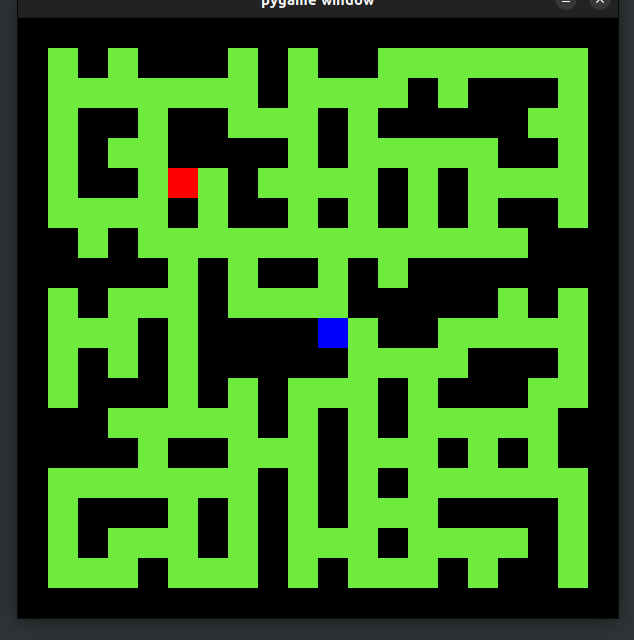
\includegraphics[width=1\textwidth]{Dissertation/Interim Report/Pictures/Mgoal.png}
         \caption*{Medium}
     \end{subfigure}
     \hfill
     \begin{subfigure}[h]{0.3\textwidth}
         \centering
         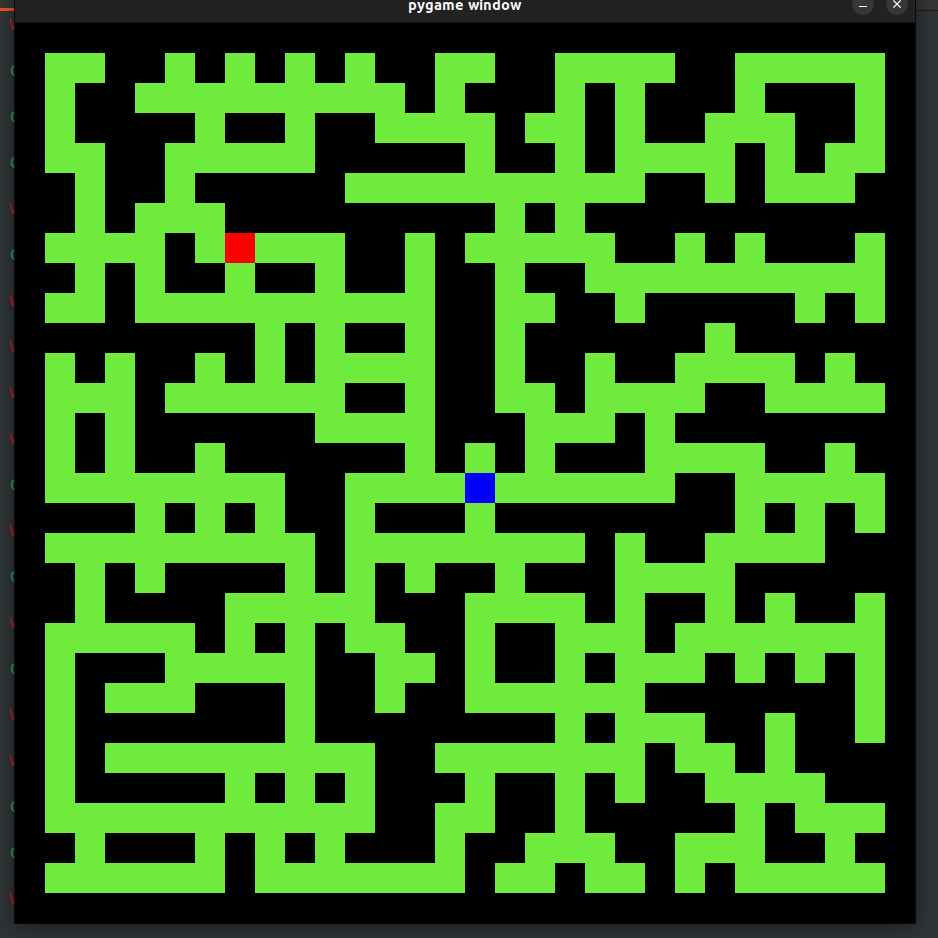
\includegraphics[width=1\textwidth]{Dissertation/Interim Report/Pictures/Lgoal.png}
         \caption*{Large}
     \end{subfigure}
        \caption{Goals marked with a red square}
        \label{fig:three graphs}
\end{figure}

\begin{center}
\begin{tabularx}{\textwidth}{ |c|| *{4}{Y|} }
 \hline
 \multirow{2}{*}{Algorithm} & \multicolumn{3}{|c|}{Average Time Taken on Maze of Size (seconds)} \\
 \cline{2-4}
  &  Small & medium & Large \\
 \hline\hline
 Breadth-First Search & 0.0335 & 0.2768 & 1.4685\\
 Depth-First Search & 0.0571 & 0.4372 & 1.5005 \\
 Depth-Limited DFS & 0.0353 & \textcolor{Emerald}{0.2298} & \textcolor{Emerald}{1.0717} \\
 Uniform-Cost Search & \textcolor{Emerald}{0.0285} & 0.3017 & 1.1334\\
 \hline
 \end{tabularx}
\end{center}
From this we can see that on average a depth-limited DFS is the fastest in this experiment. On each run it was faster than a regular DFS. This is to be expected as it doesn't search as deep as a DFS, meaning it is able to traverse more important paths quicker, thus ending up at the goal faster. On the small maze, the UCS was the quickest. This is most likely because the UCS expands very quickly in all directions whereas a DFS expands very quickly in one direction. As the maze is so small, it's not very surprising that in this case the UCS found the goal first.

%%%%%%%%%%%%%%%%%%%%%%%%%%%%%%%%%%%%%%%%%%%%%%%%%%%%%%%%%%%%%%%%%%%%%%%%%%%%%%%%%%%
\textbf{Second Experiment: Goal in corner}
\begin{figure}[h]
     \centering
     \begin{subfigure}[h]{0.3\textwidth}
         \centering
         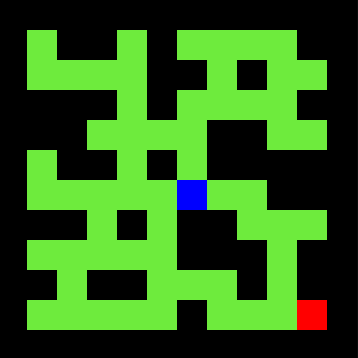
\includegraphics[width=1\textwidth]{Dissertation/Interim Report/Pictures/sCorner.png}
         \caption*{Small}
     \end{subfigure}
     \hfill
     \begin{subfigure}[h]{0.3\textwidth}
         \centering
         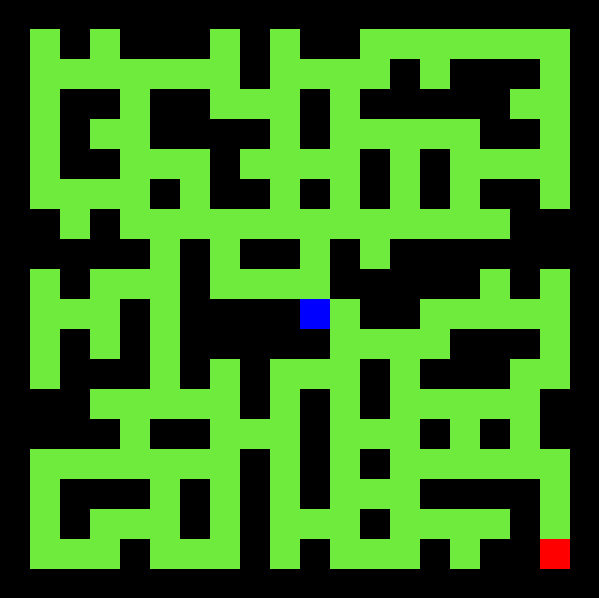
\includegraphics[width=1\textwidth]{Dissertation/Interim Report/Pictures/mCorner.png}
         \caption*{Medium}
     \end{subfigure}
     \hfill
     \begin{subfigure}[h]{0.3\textwidth}
         \centering
         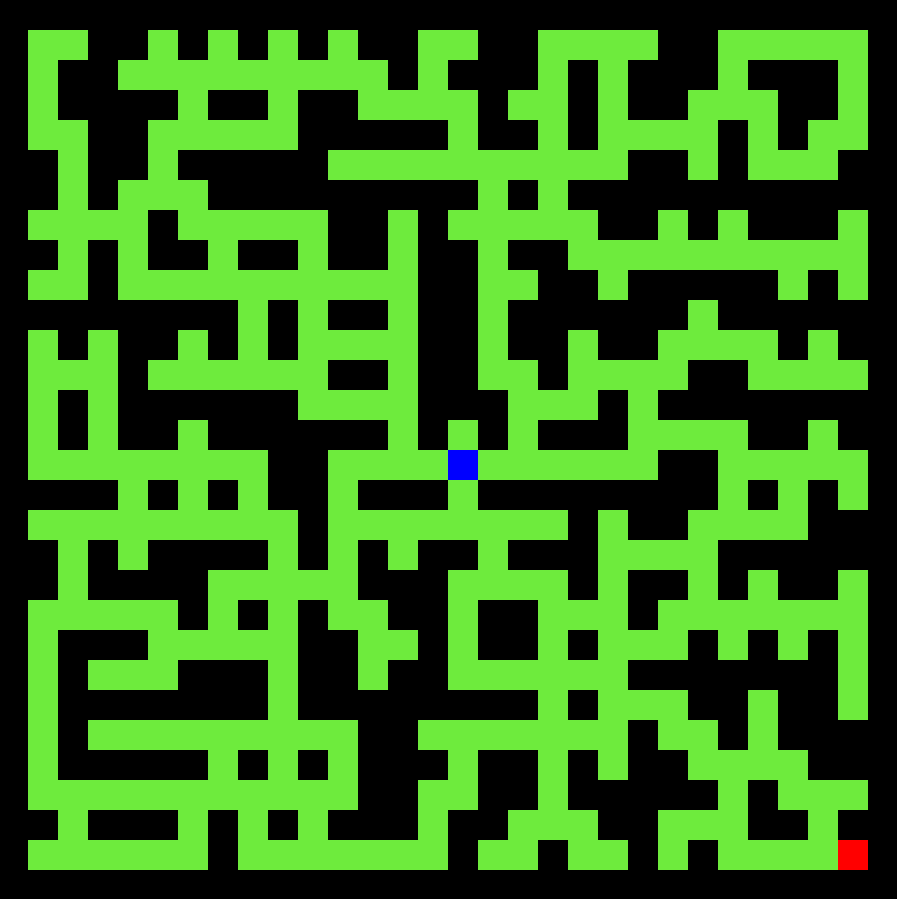
\includegraphics[width=1\textwidth]{Dissertation/Interim Report/Pictures/lCorner.png}
         \caption*{Large}
     \end{subfigure}
        \caption{Goals marked with a red square}
\end{figure}

\begin{center}
\begin{tabularx}{\textwidth}{ |c|| *{4}{Y|} }
 \hline
 \multirow{2}{*}{Algorithm} & \multicolumn{3}{|c|}{Average Time Taken on Maze of Size (seconds)} \\
 \cline{2-4}
  &  Small & medium & Large \\
 \hline\hline
 Breadth-First Search & 0.0717 & 0.5977 & 3.0384\\
 Depth-First Search & \textcolor{Emerald}{0.0152} & 0.6077 & 0.3732\\
 Depth-Limited DFS & 0.0153 & 0.5291 & \textcolor{Emerald}{0.3727}\\
 Uniform-Cost Search & 0.0587 & \textcolor{Emerald}{0.4782} & 2.551\\
 \hline
 \end{tabularx}
\end{center}

In this scenario, you would expect a DFS and depth-limited DFS to deliver the same times, as the goal is at the very edge of the map. From our results we can see this is true, with their times only differing by a few milliseconds. It is very clear when running this experiment on the large maze that a DFS and variation of is \textit{a lot} faster than a BFS or UCS. This is unsurprising as you would expect a DFS to visit a corner faster than a BFS or UCS due to the nature of the algorithm.
\newpage
%%%%%%%%%%%%%%%%%%%%%%%%%%%%%%%%%%%%%%%%%%%%%%%%%%%%%%%%%%%%%%%%%%%%%%%%%%%%%%%%%%%
\textbf{3rd Experiment: Corner to corner}
\begin{figure}[h]
     \centering
     \begin{subfigure}[h]{0.3\textwidth}
         \centering
         \includegraphics[width=1\textwidth]{Dissertation/Interim Report/Pictures/scornergoal.png}
         \caption*{Small}
     \end{subfigure}
     \hfill
     \begin{subfigure}[h]{0.3\textwidth}
         \centering
         \includegraphics[width=1\textwidth]{Dissertation/Interim Report/Pictures/mcornergoal.png}
         \caption*{Medium}
     \end{subfigure}
     \hfill
     \begin{subfigure}[h]{0.3\textwidth}
         \centering
         \includegraphics[width=1\textwidth]{Dissertation/Interim Report/Pictures/lcornergoal.png}
         \caption*{Large}
     \end{subfigure}
        \caption{Goals marked with a red square}
\end{figure}

\begin{center}
\begin{tabularx}{\textwidth}{ |c|| *{4}{Y|} }
 \hline
 \multirow{2}{*}{Algorithm} & \multicolumn{3}{|c|}{Average Time Taken on Maze of Size (seconds)} \\
 \cline{2-4}
  &  Small & medium & Large \\
 \hline\hline
 Breadth-First Search & 0.0755 & 0.6247 & 3.0858\\
 Depth-First Search & 0.0548&  \textcolor{Emerald}{0.3795} & 1.700\\
 Depth-Limited DFS &  \textcolor{Emerald}{0.0504} & 0.3811 &  \textcolor{Emerald}{1.6944}\\
 Uniform-Cost Search & 0.0734 & 0.5846 & 2.7817\\
 \hline
 \end{tabularx}
\end{center}

As in the last experiment, it would be expected that the DFS and depth-limited DFS would perform almost exactly the same, which is true once more. We can also see that as hypothesised the UCS outperformed the BFS.

In conclusion, on average the Depth-limited DFS is the quickest at finding the goal when compared to the other searches. This does of course vary based on the goal and start destination. In fact, in experiment 2 we can see that all searches are very close, if we were to scale this up to a maze size of say 50 x 50, we might find that the BFS begins to overtake as leading algorithm. In almost every case, the UCS was quicker than the BFS. This is useful for us as we care about path cost, however if we had a uniform cost for every step, the BFS would outperform our UCS, as mentioned in \ref{Search Algortithms}.

A video for the maze visualisation can be seen here: https://youtu.be/vsaYro-G3bo
%%%%%%%%%%%%%%%%%%%%%%%%%%%%%%%%%%%%%%%%%%%%%%%%%%%
\newpage
\chapter{Professional Issues}

\section{Plagiarism}

Plagiarism is the act of taking someone else's work or ideas and trying to pass them off as your own. As mentioned in section \ref{Maze implimentation}, code from the website \cite{maze} was used to help write the base for the maze generation. This could be seen as plagiarism as it is being used in our project. To make sure this won't be the case, the author and website have been referenced. The code has also been changed and edited it in the way that fits our needs, it is not purely copy and paste. It is also possible that some of the background theory could be seen as plagiarism as it has been used as research to help write about the main concepts. Wherever someone else's knowledge was used to help explain a concept, they have been cited.


%%%% ADD YOUR BIBLIOGRAPHY HERE
\newpage
\addcontentsline{toc}{chapter}{Bibliography}
\bibliographystyle{plain} % We choose the "plain" reference style
\bibliography{references} % Entries are in the references.bib file

\label{endpage}

\newpage

%TC:ignore 
\begin{appendices}
\chapter{Graph Visualisation}\label{Graph visualisation}
\begin{figure}[h]
     \caption{Graph Representation of maze}
     \centering
     \begin{subfigure}[h]{1\textwidth}
         \centering
         \includegraphics[width=0.6\textwidth]{Dissertation/Interim Report/Pictures/graph_fail1.png}
         \caption{Small Maze Graph}
         \label{fig: Small Maze graph}
     \end{subfigure}
     \hfill
     \begin{subfigure}[h]{1\textwidth}
         \centering
         \includegraphics[width=0.8\textwidth]{Dissertation/Interim Report/Pictures/graph_fail2.png}
         \caption{Large Maze}
         \label{fig: Large Maze Graph}
     \end{subfigure}
\end{figure}

I attempted to use the python libraries matplotlib and networkx to represent the nodes in the maze as a graph, however I quickly realised this was a bad idea. Although the figure \ref{fig: Small Maze graph} is somewhat readable it is not very clear which nodes connect to each other due to the overlapping edges. To see if this as fixable i did some research, after not finding a solution and given this is not a vital piece of material, I decided to leave it out. It seems that the visualisation of the large maze in figure \ref{fig: Large Maze Graph} would be complex to read regardless given the size.
\end{appendices}
%TC:endignore 
\end{document}

\end{article}


